
% FILE: figures/raf_network.tex
% RAF network schematic

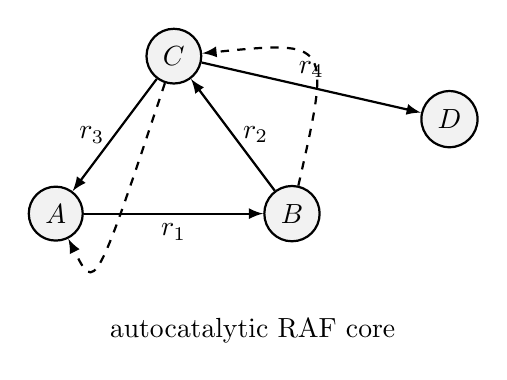
\begin{tikzpicture}[>=latex,thick,scale=1]
  % Molecules
  \node[draw, circle, fill=gray!10] (A) at (0,0) {$A$};
  \node[draw, circle, fill=gray!10] (B) at (3,0) {$B$};
  \node[draw, circle, fill=gray!10] (C) at (1.5,2) {$C$};
  \node[draw, circle, fill=gray!10] (D) at (5,1.2) {$D$};

  % Reactions
  \draw[->] (A) -- (B) node[midway,below] {$r_1$};
  \draw[->] (B) -- (C) node[midway,right] {$r_2$};
  \draw[->] (C) -- (A) node[midway,left] {$r_3$};
  \draw[->] (C) -- (D) node[midway,above] {$r_4$};

  % Catalytic edges
  \draw[dashed,->] (C) .. controls (0.5,-1.0) .. (A);
  \draw[dashed,->] (B) .. controls (3.5,2.2) .. (C);

  \node[anchor=north] at (2.5,-1.2) {autocatalytic RAF core};
\end{tikzpicture}
